% ============================================================================
% 中文注释：CVPR 2027 投稿主文件
% ----------------------------------------------------------------------------
% 模板：官方 author-kit（cvpr-org/author-kit），cvpr.sty 与 ieeenat_fullname.bst 原样使用。
% 当前模式：\usepackage[review]{cvpr} —— 匿名评审版（页眉显示 CONFIDENTIAL REVIEW COPY、
%           正文带行号、作者栏为 Anonymous）。投稿时不要改成 camera-ready。
% 结构：
%   sec/0_abstract     摘要（三条发现）
%   sec/1_intro        引言 + teaser 四联图
%   sec/2_related      相关工作
%   sec/3_benchmark    采集协议 / 面板 / 指标 / AE 与错位两个陷阱
%   sec/4_diagnosis    ★核心：两条失败轴 + "功臣不是区域语义"
%   sec/5_method       L_quiet（无掩码的改变化感知正则）
%   sec/6_experiments  主表 / L_quiet / 哪项吃重 / 域消融 / 负结果
%   sec/7_conclusion   局限、采集 checklist、诚实声明
%   tab/main_table     表 1（跨栏）
%   tab/negative       表 2（负结果）
% 篇幅：正文 6 页 + 参考文献 1 页 = 7 页（CVPR 限 8 页，不含参考文献）。
% 构建：.\build.ps1（本地 TinyTeX）或 Overleaf（pdfLaTeX）。
% 切换：
%   相机就绪版 → \usepackage{cvpr}，并补作者块
%   arXiv 带页码 → \usepackage[pagenumbers]{cvpr}
% ============================================================================
% CVPR 2027 submission — anonymous review version
\documentclass[10pt,twocolumn,letterpaper]{article}

%%%%%%%%% PAPER TYPE
\usepackage[review]{cvpr}      % review (anonymous) version
% \usepackage{cvpr}            % camera-ready
% \usepackage[pagenumbers]{cvpr}

%% Preamble for the CVPR 2027 submission (based on the official author kit)
% \usepackage{cuted}  % 不用 strip 环境；cuted 会干扰普通 float 的排版（实测导致表格叠字）
% \usepackage{currfile}  % 未用 \currfilebase
\usepackage{caption}
\usepackage{amsmath,amssymb,amsthm,bm}
\usepackage{graphicx}
\usepackage{booktabs}
\usepackage{multirow}
\usepackage{array}
\usepackage{xcolor}
\usepackage{siunitx}

\newtheorem{proposition}{Proposition}
\newtheorem{definition}{Definition}

\DeclareMathOperator*{\argmin}{arg\,min}
\DeclareMathOperator*{\argmax}{arg\,max}

\newcommand{\Om}{\Omega}
\newcommand{\dOm}{\partial\Omega}
\newcommand{\T}{\mathbf{T}}
\newcommand{\I}{\mathbf{I}}
\newcommand{\R}{\mathbf{R}}
\newcommand{\That}{\widehat{\mathbf{T}}}
\newcommand{\Rhat}{\widehat{\mathbf{R}}}
\newcommand{\Lhalf}{\mathcal{L}}
\newcommand{\quiet}{\mathcal{L}_{\mathrm{quiet}}}
\newcommand{\reg}{\mathcal{L}_{\Om}}
\newcommand{\dBA}{\,\mathrm{dB}}
\newcommand{\PSNOm}{\mathrm{PSNR}_{\Om}}
\newcommand{\PSNOut}{\mathrm{PSNR}_{\bar\Om}}

\newcommand{\red}[1]{{\color{red}#1}}
\newcommand{\todo}[1]{{\color{red}#1}}

%% Shrink the reference list slightly (does not affect the 8-page body limit,
%% but keeps the PDF readable while drafting).
% 不覆盖参考文献字号：CVPR 规定字号由模板控制，手工压缩属拒稿条款


\definecolor{cvprblue}{rgb}{0.21,0.49,0.74}
\usepackage[pagebackref,breaklinks,colorlinks,allcolors=cvprblue]{hyperref}

\def\confName{CVPR}
\def\confYear{2027}

%%%%%%%%% TITLE
\title{What Single-Image Reflection Removal Does to the Occluder Region:\\[2pt]
A Diagnostic Benchmark on Tinted Glass}

%%%%%%%%% AUTHORS (anonymized for review)
\author{Anonymous submission\\Paper ID ****}

\begin{document}
\maketitle

% ============================================================================
% 中文注释：摘要（Abstract）—— 2026-11-03 按"贴膜玻璃是独立物理体制"重写
% ----------------------------------------------------------------------------
% 叙事顺序：
%   ① 普通 SIRR 的隐含假设：反射鲜明、透射清晰 ⇒ 主要矛盾是"分离"
%   ② 贴膜玻璃破坏了这个前提：膜是暗色的，两层同时被衰减 ⇒ 主要矛盾变成
%      "暗反射 + 低信噪透射 + 二者同频段" ⇒ 不是分离问题，而是辨识问题
%   ③ 由此得到四条可测失败模式（每条带数字）
%   ④ 采集层面的连带问题：黑布法引入系统性光照差 ⇒ 光度对齐与去反射必须统一
%   ⑤ 我们给的两件事：一个无掩码正则（+0.50 dB）+ 一套诚实的负结果与探针
% 关键数字：
%   反射/透射 = 0.201（Ω 外） / 0.112（Ω 内）；反射能量 34.5% 在高频
%   暗处反射扰动比亮处高 64%（23.06 vs 14.07 灰阶）
%   Ω 内 identity 24.52 dB 最高；公开方法 20.9–23.6；我们 22.39
%   Ω 内结构保有率：模型 0.48–0.65（GT=1）
%   逐图仿射 oracle 0.15–0.26 dB vs 留一场景共享 0.07 dB
%   L_quiet: +0.50 dB，95% CI [+0.34,+0.67]，14/15 场景为正
% 注意：Ω 内"透射被压暗"在 1019 面板上是 0.987（≈不变），只有 165530 是 0.830，
%       ⇒ 不要写成普适规律，写成"分场景、非系统性"。
% ============================================================================
\begin{abstract}
% 中文：普通 SIRR 假设"反射鲜明、透射清楚"，于是问题是分离。
Single-image reflection removal (SIRR) implicitly assumes a friendly photometric
regime: the reflected scene is bright, the transmitted scene is well exposed, and the
task is to \emph{separate} two comparable layers.

% 中文：贴膜玻璃破坏了这个前提——膜是暗色的，两层同时被压低。
We show that \textbf{tinted window film destroys this premise}. The film is dark: it
attenuates the reflected layer \emph{and} the transmitted layer at the same time. On a
hand-annotated $15$-scene panel shot through automotive window film we find that the film
treats the two layers \emph{differently}: the transmitted layer passes through the film bulk and
is scattered and dyed, while the reflection comes off the film surface. The result is a layer
asymmetry---the transmission is $2.3\times$ softer than on ordinary glass and the reflection is
$2.0\times$ sharper relative to it---which is \emph{not} explained by brightness: mean levels,
reflection magnitude and spectral overlap all match Real20. Under such a regime SIRR is not a
separation problem but an \emph{identification} problem.

% 中文：四条可测失败模式。
This reframing yields four measurable failure modes. (i)~The reflection is \emph{not}
strongest inside the occluder region $\Om$ but in the annulus around it: $4.3\times$ stronger than
inside $\Om$, covering $44\%$ of the frame, and that annulus is where every model is worst
($19.4$--$19.8\dBA$ vs.\ $23.5$ far away). Inside $\Om$ almost nothing needs to change yet every
method is worse than doing nothing (identity $24.52\dBA$ vs.\ $20.9$--$23.6$ for six public
methods and $22.4$ for ours), so the residual is read as a \emph{boundary}. (ii)~The damage is not a
photometric offset: after a per-image affine correction the models retain only
$0.48$--$0.65$ of the ground-truth structure inside $\Om$. (iii)~The reflection and the
scene share the same frequency band, so simply restoring the input's high frequencies
\emph{lowers} PSNR---faithful recovery requires semantic priors, not better filtering.
(iv)~What survives fine-tuning is per-image: a per-image affine oracle recovers
$0.15$--$0.26\dBA$ whereas a single shared affine fitted on other scenes recovers
$0.07\dBA$.

% 中文：采集层面的连带问题。
The standard ground-truth protocol---covering the glass with dark cloth---adds a
systematic illumination change, so photometric alignment and reflection removal cannot be
treated separately.

% 中文：我们给的东西 + 诚实边界。
We give a region-relative loss that is load-bearing ($-4.2\dBA$ if removed), a mask-free
change-aware regularizer derived from a random-disk control ($+0.50\dBA$, per-scene
$95\%$ CI $[+0.34,+0.67]$, positive on $14/15$ scenes, zero inference cost), and a
systematic set of negative results including perceptual losses, high-frequency splicing
and data mixing.
\end{abstract}

% ============================================================================
% 中文注释：第 1 节 引言（2026-11-03 第三版）——按标准论文结构重写
% ----------------------------------------------------------------------------
% 结构（用户指定）：
%   ① 背景：SIRR 是什么、用在哪些场景、主流方法解决了什么
%   ② 痛点：真实部署里玻璃基本都贴膜；贴膜改变的成像；现有方法因此失效
%   ③ 前人方法：做过什么、进展到哪、仍缺什么
%   ④ 自己方法 + teaser（图 1 = 同权重 Real20 成功 / 贴膜失败）
%   ⑤ 核心贡献 5 条 bullet（数据 / 成像 / 区域分析 / 方法 / 负结果）
%   ⑥ 论文结构
% 写作纪律（用户要求）：
%   **intro 不写具体数字**，数字一律留给图表。
%   数据贡献必须写全：15 场景测试集 + 4/5/6/11 月四个训练批次。
% ============================================================================
\section{Introduction}
\label{sec:intro}

% 中文：图 1 —— 同一官方权重（RDNet CVPR'25），Real20 能去干净、贴膜场景去不掉。
\begin{figure*}[t]
\centering
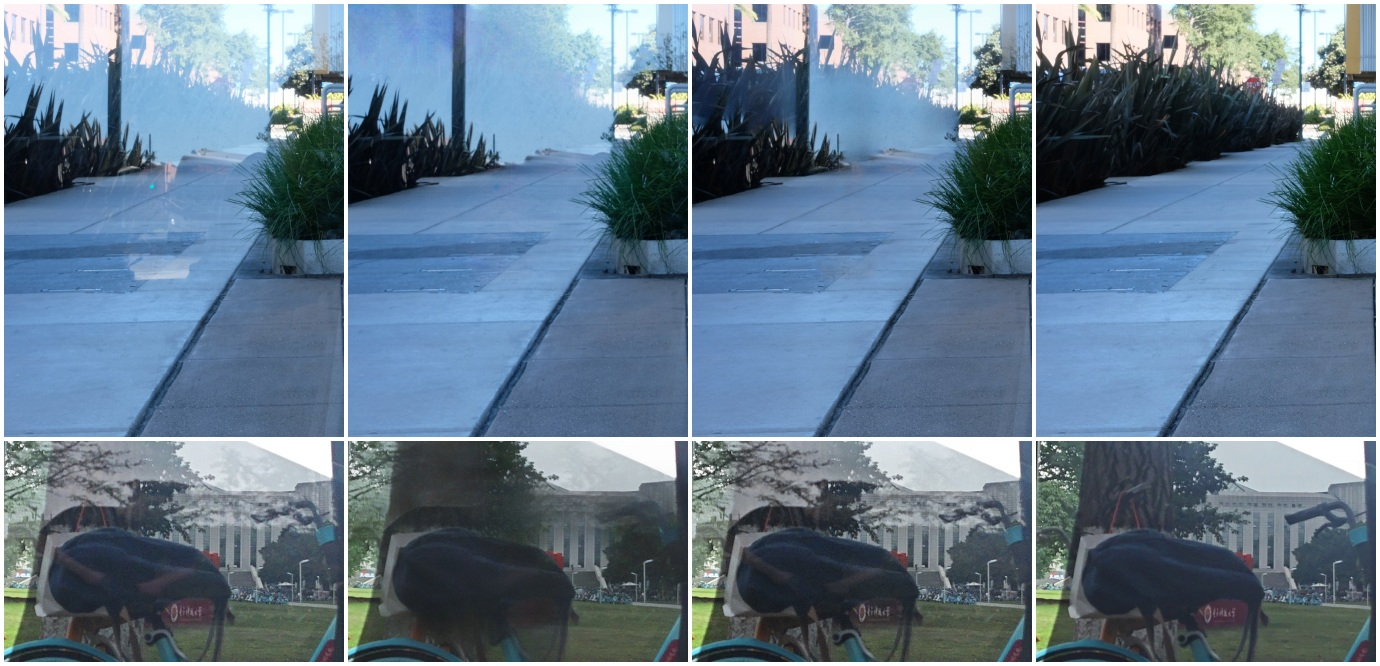
\includegraphics[width=0.86\textwidth]{fig/teaser_2rows.jpg}
\caption{\textbf{Same models, two kinds of glass.} Top, on a standard benchmark (Real20): the
state-of-the-art method~\cite{rdnet25} removes the reflection almost completely, while a second
recent method (LightRR~\cite{lightrr26}) removes only part of it. Bottom, on a pair from our
filmed-glass panel: the \emph{same} RDNet does not remove the reflection at all---instead it darkens
the frame and strips transmitted detail---and LightRR changes almost nothing. The difference is not
the network but the imaging: window film is laminated on the scene side, so the transmitted light
passes through the film while the reflection of the behind-camera environment does not. The two
layers end up separated in \emph{band} rather than in \emph{level}, and a model trained on ordinary
glass misreads what to take away.}
\label{fig:teaser}
\end{figure*}

% 中文：① 背景。
Single-image reflection removal (SIRR) addresses a situation everyone with a camera has met: a
photograph taken through a pane of glass, in which the scene behind the camera is superimposed on
the scene in front of it. The setting is ubiquitous---car windows, shop and office facades, museum
cases, aquaria---and the degradation is severe enough that SIRR has become a standing task in
computational photography. The dominant recipes are now data-driven: large paired corpora of
``with reflection / without reflection'' images, a network that regresses the transmitted layer, and
an objective that penalises the difference from the clean reference. Classical layer priors gave way
to cascaded and recurrent designs, then to reversible and dual-stream architectures, and each
generation has advanced the state of the art on benchmarks such as Real20 and SIR$^2$.

% 中文：② 痛点。真实部署 = 贴膜玻璃。
What these recipes share is an implicit assumption about the \emph{glass}. In deployment the glass
is rarely bare: automotive and architectural glazing is almost always \emph{filmed}, for heat
rejection, privacy and UV protection. A dark film changes the imaging in a way that the standard
assumption does not cover. The film sits on the scene side, so the light we want must travel through
it---and is scattered, absorbed and tinted on the way---while the light we want to discard comes off
the bare surface facing the camera and passes through nothing. The observed image is therefore not a
bright reflection layered on a well-exposed scene, but a \emph{sharp} reflection over a \emph{soft},
desaturated transmission. Methods trained on ordinary glass, and evaluated on ordinary glass, have no
reason to expect this, and empirically they do not survive it (Fig.~\ref{fig:teaser}).

% 中文：③ 前人方法：做过什么、缺什么。
The community has of course attacked the difficulty of SIRR from several directions: stronger
backbones and attention, reversible or invertible connections to preserve information, explicit
estimates of the reflection rate, physics-inspired layer decompositions, and larger or more realistic
synthetic corpora. What these efforts have in common is where they are measured: on benchmarks whose
reflections are \emph{dense}, covering most of the frame, so that an average error over the image is
already a faithful description of the failure. Three things are consequently missing. There is no
real paired dataset shot through filmed glass, so the regime cannot even be measured. There is no
analysis of \emph{where} a method fails---strong reflection is not distributed uniformly over the
frame, and a single average number cannot distinguish the regions where removal is necessary from
those where it is harmful. And because no such analysis exists, the losses used in training are
inherited from dense-reflection settings, where they work.

% 中文：④ 自己方法：先量清楚，再给监督。
This paper takes the opposite order. We first ask what filmed glass actually does to the two layers,
and answer it with measurements: the transmission loses high-frequency content relative to ordinary
glass while the reflection does not, so the layer that carries the detail and the layer that must be
discarded are separated in frequency rather than in brightness. We then ask \emph{where} current
methods fail, and find that the answer is unintuitive: the reflection is weakest exactly in the
region the eye fixates on---the patch where a dark object of the reflected environment projects,
which we call the low-change region---and strongest in the annulus immediately around it. The
annulus is large, its transmitted content is buried, and every model we tested is worse there than
anywhere else in the frame; because it borders a region that is already almost correct, its residual
error is read by the eye as a boundary. Finally, guided by this picture, we design the training
signal: a compact region with a large weight is what keeps a sparse reflection from being
under-weighted by the global objective, and this can be obtained without any annotation at all.
Along the way we capture the data that makes the analysis possible.

% 中文：⑤ 核心贡献。
\paragraph{Contributions.}
\begin{itemize}
\item \textbf{Data.} A real-pair benchmark for filmed glass: a hand-annotated test panel of
$15$ scenes, and training pairs captured in four sessions (April, May, June and November) on the
same rig with exposure and white balance locked. We also report the two capture pitfalls that
silently ruin such data---unlocked auto-exposure, which makes the ``clean'' reference a different
exposure of the scene, and misalignment between the pair---together with the protocol we use to
avoid them.
\item \textbf{Imaging.} A measurement-based account of filmed glass as a layer \emph{asymmetry}:
transmission through the film bulk, reflection off the bare surface. We show that the two layers
differ in band and in chroma, but not in mean level, which distinguishes filmed glass from ordinary
glass and explains why off-the-shelf models transfer poorly.
\item \textbf{Regional analysis.} A decomposition of the failure into the low-change region and the
annulus around it. The reflection is weakest inside the region and strongest in the annulus; models
are worse than doing nothing inside the region, and at their absolute worst in the annulus. This is
what makes the boundary, rather than either region on its own, the thing one sees.
\item \textbf{Method.} Evidence that region-relative supervision is load-bearing for sparse
reflection, and a mask-free change-aware regulariser, $\mathcal{L}_{\mathrm{quiet}}$, derived from
it: no annotation, no parameters, no inference cost, and a consistent improvement over our
fine-tuning baseline.
\item \textbf{Negative results.} A systematic account of what does \emph{not} work on this problem,
with a mechanism for each failure: perceptual losses, restoring the input's high frequencies,
mixing in more in-domain data, a photometric adapter, a residual gate, and a dual-dictionary
separation probe.
\end{itemize}

% 中文：⑥ 论文结构。
\paragraph{Organisation.}
Sec.~\ref{sec:related} reviews related work. Sec.~\ref{sec:benchmark} describes the imaging of
filmed glass, the capture protocol and the datasets. Sec.~\ref{sec:diagnosis} analyses where and why
current methods fail. Sec.~\ref{sec:method} derives the training signal, and
Sec.~\ref{sec:experiments} reports results, ablations and negative results.
Sec.~\ref{sec:conclusion} discusses limitations and the open problem of completing the annulus.

% ============================================================================
% 中文注释：第 2 节 相关工作（Related Work）
% ----------------------------------------------------------------------------
% 四段，每段只讲"与我们相关的差异"，不复述别人的方法细节：
%   ① 经典/深度 SIRR：都按平均 PSNR 报，没人报"Ω 内是否变差"。
%   ② 基准与盲点：拿 T 的三种做法（移走反射源/偏振/盖布）都会改变采集，
%      且没有记录"反射在哪里被压掉了"——这是本文补的。
%   ③ 归纳偏置架构（可逆/提示/频域/prompt）：数据少时容易把先验过拟合；
%      §6 里两个这类方案是被 CPU 探针在训练前否掉的。
%   ④ 光度一致性（Retinex/低光）：对应本文的第二条失败轴，§4.2 证明它逐图、不可共享。
% 注意：引用里 DSRNet / Zhu24 / LightRR / wavelet 目前是占位条目，投稿前必须替换。
% ============================================================================
\section{Related Work}
\label{sec:related}

% 中文：经典方法用梯度稀疏/层先验；深度方法直接回归透射层。
% 共同点：全部按平均 PSNR/SSIM 在 Real20、SIR² 或自建划分上报。
\paragraph{Single-image reflection removal.}
Classical approaches exploit gradient sparsity and layer priors
\cite{levin04,li13,wan17}; deep methods regress the transmission layer directly
\cite{fan17,zhang18,wei19,hu20}. ERRNet~\cite{wei19} aligns misaligned training pairs; IBCLN~\cite{li20}
uses a cascaded bidirectional loop; DSRNet~\cite{dsrnet24} introduces dual-stream interaction; and
RDNet~\cite{rdnet25}, the NTIRE~2025 challenge winner, replaces U-Net connections by a multi-column
\emph{reversible} encoder and conditions on an estimated transmission rate. Zhu~\cite{zhu24}
explores layer-separation priors. All of these are evaluated by average PSNR/SSIM on
Real20~\cite{zhang18}, SIR$^2$~\cite{wan17} (Objects/Postcard/Wild) or their own splits.

% 中文：真配对数据很贵；拿 T 的三种做法都会改变采集，且都没记录"反射在哪里被压掉"。
% 指标算全图 ⇒ 紧凑区域的失效被稀释。我们的面板显式标注这个区域并要求分区报告。
\paragraph{Benchmarks and their blind spots.}
Real paired SIRR data is expensive: one has to obtain the same scene with and without reflection.
Existing protocols obtain $T$ by (a)~moving the reflection source out of view, (b)~using a
polariser, or (c)~covering the glass. Each changes the acquisition, and none of them records
\emph{where} the reflection was suppressed. Metrics are therefore computed over the whole image,
which dilutes a spatially compact failure. Our panel explicitly annotates the suppressed region and
reports it separately.

% 中文：可逆连接、传输率提示、频域分解、prompt 条件化——这些先验在数据充足时有价值；
% 数据只有几个场景时容易把先验本身过拟合。§6.5 报了两个被探针提前否掉的方案。
\paragraph{Inductive-bias architectures.}
A recent trend is to inject structural assumptions: reversible/invertible connections to avoid
information loss~\cite{revcol,rdnet25}, transmission-rate prompts~\cite{rdnet25}, frequency or
wavelet decomposition~\cite{wavelet}, and prompt-conditioned multi-task restoration~\cite{promptir}.
Such priors are valuable when the data regime allows the prior to be identified; with a handful of
scenes it is easy to over-fit the prior instead. Sec.~\ref{sec:experiments} reports two such
proposals that our CPU probes rejected before training.

% 中文：Retinex/低光路线会预测逐图增益；在 SIRR 里对应的量是 I 与 T 的全局光度偏移。
% §4.2 证明：微调后这个量几乎被吃干，且剩余部分逐图、无法用共享规则预测。
\paragraph{Photometric consistency in restoration.}
Retinex-style and illumination-aware methods~\cite{retinexformer} model a global light field, and
low-light work routinely predicts a per-image gain. For SIRR, the analogous quantity is the global
photometric offset between $I$ and $T$; Sec.~\ref{sec:diagnosis} shows that after fine-tuning this
quantity is (a)~almost exhausted by training and (b)~per-image, so it cannot be predicted from a
single frame by any shared rule.

% ============================================================================
% 中文注释：第 3 节 贴膜玻璃：光度、协议、面板（2026-11-03 重写）
% ----------------------------------------------------------------------------
% 这一节的任务：把"贴膜玻璃是独立物理体制"从说法变成数字。
%   3.1 膜的成像效应（P1/P2）：反射只占透射 20.1%；反射 34.5% 在高频；
%       暗处反射扰动比亮处大 64%（23.06 vs 14.07 灰阶）。
%   3.2 采集协议与 GT 的危险（P4）：黑布法改光照；AE 状态必须报。
%   3.3 面板与指标：15 场景、手标 Ω（中位 4.6%，2.9–9.2%）、β/α 两个诊断标量。
% 数据出处（服务器）：
%   probe_tinted_photometry_1103.py（P1/P2 数字）
%   remeasure_alpha_annot_1102.py（∂Ω 梯度）
%   qa_split.csv（Ω 面积分布）
% ⚠️ 注意：Ω 内透射被压暗在 1019 上是 0.987（≈不变），只有 165530 是 0.830，
%      所以文中写"分场景、非系统性"，不要写成普适规律。
% ============================================================================
\section{Tinted Glass: Photometry, Protocol, Panel}
\label{sec:benchmark}

% 中文：3.1 膜做了什么——三个可测的量。
\subsection{What the film does to the two layers}
\label{sec:film}

Consider the sensor measurement through a filmed pane,
\begin{equation}
I(x) \;=\; \tau\,T(x) \;+\; \rho\,R(x),
\label{eq:film}
\end{equation}
where $\tau$ is the (film-attenuated) transmission, $\rho$ the reflection coefficient, $T$
the scene and $R$ the reflected scene. Ordinary SIRR implicitly assumes $\rho R$ is
\emph{bright} and $\tau T$ is \emph{well exposed}. Window film inverts both. We measure
three consequences.

% 中文：P1 暗反射。
% 中文：P1 改为"锐度/色度不对称"——这是与 Real20/SIR² 相比真正有 2 倍差异的量。
\paragraph{P1 --- the two layers are not equally sharp.}
The film is laminated on the scene side and the camera is on the bare side, so the two layers
traverse the film differently: transmitted light passes \emph{through} the film bulk (scattered,
absorbed, dyed), whereas the reflection of the behind-camera environment comes off the bare
\emph{glass surface} and never enters the film at all. The prediction is a layer
asymmetry in sharpness and chroma, and this is what we observe. Measured per pair with
$\mathrm{sharp}(X)=\mathbb{E}|\mathrm{HP}(X)|/\mathbb{E}|X|$ (HP: unit-variance high-pass) and
averaged over each dataset:

\begin{center}
\small
\setlength{\tabcolsep}{4pt}
\begin{tabular}{@{}lcccc@{}}
\toprule
 & Real20 & SIR$^2$-Obj & SIR$^2$-Wild & \textbf{ours (film)} \\
\midrule
$\mathrm{sharp}(T)$ & $0.062$ & $0.054$ & $0.041$ & $\mathbf{0.027}$ \\
$\mathrm{sharp}(R)/\mathrm{sharp}(T)$ & $3.32$ & $2.51$ & $2.58$ & $\mathbf{6.76}$ \\
chroma of $T$ & $0.373$ & $0.322$ & $0.393$ & $\mathbf{0.219}$ \\
\bottomrule
\end{tabular}
\end{center}

The transmitted layer of filmed glass is $2.3\times$ softer than on ordinary glass and its
reflection is $2.0\times$ sharper \emph{relative to it}. Mean brightness, mean reflection
magnitude and the high-frequency \emph{fraction} of the reflection are, by contrast,
indistinguishable from Real20 (all measured identically on the four datasets); the asymmetry is what separates the two
regimes.

\paragraph{P2 --- dark content is hit hardest.}
Sorting the scene pixels of each frame by their ground-truth luminance and averaging the
reflection magnitude $|I-T|$ within each quartile gives

\begin{center}
\small
\setlength{\tabcolsep}{4pt}
\begin{tabular}{@{}lcccc@{}}
\toprule
scene luminance & Q1 (dark) & Q2 & Q3 & Q4 (bright) \\
\midrule
mean $|I-T|$ & $\mathbf{23.1}$ & $25.7$ & $17.7$ & $14.1$ \\
\bottomrule
\end{tabular}
\end{center}

The reflection perturbs the darkest quartile $64\%$ more than the brightest. The film
therefore degrades the two layers \emph{in the same places}: where the transmission is
weakest, the relative contribution of the reflection is largest. This is the opposite of
the usual SIRR setting, where a bright reflected scene sits on top of a well-exposed one.

% 中文：P3 透射层信息量低 + 需要注意的口径。
\paragraph{P3 --- the transmission loses information, unevenly.}
Inside $\Om$ the transmitted level relative to $T$ is $0.987$ on average, i.e.\
\emph{not} systematically darker on our panel; the effect is scene-dependent
(min $0.830$ for the darkest case, max $1.046$). We therefore do not claim a universal
darkening inside $\Om$. What is systematic is the loss of \emph{usable} transmitted
detail: inside $\Om$ our models retain only $0.48$--$0.65$ of the ground-truth structure
(Sec.~\ref{sec:structural}), and the strongly-reflected subset carries so little
information that a plain Gaussian blur of the input outperforms every model we trained
(Sec.~\ref{sec:ceiling}).

% 中文：3.2 采集协议与 GT 危险（P4）。
\subsection{Capture protocol and the ground-truth hazard}
\label{sec:protocol}

All scenes are shot on a phone through an automotive window film, handheld, with exposure
and white balance \emph{locked}. For each scene we record a short clip with reflection and
then cover the glass with dark cloth to obtain $T$. There is \textbf{one $T$ per scene}
and many $I$; inputs are extracted at $30$\,fps and cropped to the glass area, and a pair
is kept only if the phase-correlation shift is $\le1.5$\,px and the per-channel gain
deviation is $\le0.10$.

% 中文：P4：黑布法不只是"去掉反射"，它同时改光照。
\paragraph{P4 --- covering the glass is not a neutral operation.}
Covering the pane removes the reflection \emph{and} changes the light reaching the scene;
on filmed glass, where the transmitted signal is already weak, this perturbation is not
negligible relative to the reflection itself. Two practical consequences follow.
\emph{(a) Exposure must be locked}: with auto-exposure active we measured
$\mathrm{median}(I/T)=0.99$ (the covered frame was \emph{brighter}) and a residual layer
correlated with image brightness at $r=0.32$; after locking, $r=-0.01$. \emph{(b) The
residual photometric error must be re-measured, not assumed}: Sec.~\ref{sec:photometric}
shows it is per-image and cannot be shared across scenes. Photometric alignment and
reflection removal therefore have to be handled jointly, and any SIRR benchmark that
reports only pair counts is under-specified.

% 中文：3.3 面板与指标。
\subsection{Panel and metrics}
\label{sec:panel}

The panel contains $15$ scenes ($1280{\times}832$), all outdoor, all shot through the filmed pane
with the reflected environment visible. For every scene we hand-annotated $\Om$ once (median $4.6\%$
of the image, range $2.9$--$9.2\%$). By construction (Sec.~\ref{sec:protocol}) $\Om$ is the
projection of a \emph{dark} object of the reflected environment: the reflection contributes little
there, so $I$ already equals the transmitted layer and a method should only undo the film. Pixels of
the annotated polygon whose transmission deficit is large ($|I-T|>15$) belong to \emph{strong}
reflection rather than to $\Om$; we keep them as a separate \emph{shade} class instead of folding
them in, and report the annulus around $\Om$ separately in Sec.~\ref{sec:axis1}.

We report PSNR, SSIM, HF-PSNR, gradient cosine and the Laplacian-variance ratio
$\mathrm{LapVar}(\That)/\mathrm{LapVar}(T)$, plus region-restricted PSNR inside and outside
$\Om$, and two diagnostic scalars: the residual-reflection coefficient
$\beta=\langle T-\That,\,I-T\rangle/\lVert I-T\rVert^2$ ($-1$: nothing removed, $0$:
perfect) and the per-image gain
$\alpha=\mathrm{median}_i(\overline{\That_i}/\overline{T_i})$, which exposes models that
merely brighten or darken the frame.

% ============================================================================
% 中文注释：第 4 节 失败模式（2026-11-03 重写为四小节 + 区域项）
% ----------------------------------------------------------------------------
% 4.1 Ω 内所有方法劣于不作处理（表 1 + 图 2）
% 4.2 损伤是"结构"不是"光度"；而且没有任何方法打赢"无内容先验的平滑上限"
% 4.3 反射与场景同频段 ⇒ 搬高频反而掉分（解释为什么滤波/感知都无效）
% 4.4 残余光度误差是逐图的、不可跨场景迁移（P4 的量化）
% 4.5 起决定作用的损失项不是"区域"，而是"相对归一"（随机盘对照）
% 关键数字：
%   identity 24.52；公开 20.9–23.6；我们 22.30/22.39
%   结构保有率 identity 1.14 / quiet 0.65 / 50:50 0.48
%   MAE_aff identity 10.51 / quiet 11.70 / 50:50 10.71
%   平滑上限：弱区 29.50（identity 31.45，quiet 27.18）；强区 15.24（identity 14.46，quiet 13.48）
%   高频拼接：quiet 22.26→22.04(σ=2)→21.66(σ=4)；50:50 23.73→23.39
%   Δaff：identity 1.94 / RDNet 1.00 / 我们 0.15–0.26；共享 0.50 / 0.59 / 0.07
%   λ_om=0 → 18.33；随机盘 19.90 > 真掩码 19.41 > 无区域项 17.76
% ============================================================================
\section{Where SIRR Fails on Tinted Glass}
\label{sec:diagnosis}

% ============================================================================
% 中文注释：表 1 主结果（跨双栏 table*）
% ----------------------------------------------------------------------------
% 口径：15 场景、**手标 Ω** 掩码、存盘 uint8 PNG、同一冻结评测脚本。
% 行：
%   identity            —— 什么都不做（分数地板）；Ω 内 24.52 是全场最高，这是本文的核心事实
%   IBLCN / ERRNet / LightRR / RDNet(0-shot) / DSRNet / Zhu24 —— 六个公开方法，全部零样本
%   Ours (baseline)     —— 我们的 9 项损失基线，三种子 22.49±0.44
%   Ours + L_quiet      —— 本文的方法，三种子 22.99±0.34
% 列说明：
%   ΔΩ = PSNR_Ω(方法) − PSNR_Ω(identity)，**全是负的**（=所有方法都在 Ω 内比不动更差）
%   β  = 残留反射系数（−1 没去、0 完美）；公开方法的预测我们没有 R 分支，故留 "—"
%   α  = 逐图增益中位数（1 = 亮度对；偏离说明模型只是在整体提亮/压暗）
% 注意：
%   1) Ω 内/外的绝对值不可直接比（Ω 更暗、PSNR 偏爱暗区），必须看 ΔΩ；
%   2) 最佳值加粗：PSNR_Ω 与 ΔΩ 用 identity，PSNR 用我们的 L_quiet；
%   3) 细节指标（HF-PSNR、梯度余弦、LapVar）用来防"糊出来的 PSNR"——我们的 LapVar 只有 GT 的 0.6。
% ============================================================================
\begin{table*}[t]
\centering
\caption{Main results on the $15$-scene tinted-glass panel. $^\dagger$: three seeds,
mean$\pm$sd over scenes. $\Delta_\Om$ is measured \emph{against identity inside $\Om$}
(Eq.~1); it is negative for every method. $\beta$: residual-reflection coefficient
($-1$: nothing removed, $0$: perfect). $\alpha$: median per-image gain. The best value in each
column is in bold.}
\label{tab:main}
\setlength{\tabcolsep}{4pt}
\small
\begin{tabular}{lcccccccc}
\toprule
Method & PSNR$\uparrow$ & SSIM$\uparrow$ & HF-PSNR$\uparrow$ & grad-cos$\uparrow$ & LapVar & PSNR$_\Om\uparrow$ & $\Delta_\Om$ & $\beta$$\downarrow$ \\
\midrule
Identity (no removal)      & 18.44 & 0.693 & 32.96 & 0.599 & 52.5 & \textbf{24.52} & $0.00$ & $-1.00$ \\
IBLCN~\cite{li20}          & 18.12 & 0.683 & 32.68 & 0.582 & 61.0 & 23.55 & $-0.97$ & --- \\
ERRNet~\cite{wei19}        & 18.90 & 0.710 & 33.64 & 0.614 & 25.8 & 22.97 & $-1.55$ & --- \\
LightRR~\cite{lightrr26}   & 19.18 & 0.680 & 32.34 & 0.594 & 68.8 & 20.89 & $-3.63$ & --- \\
RDNet~\cite{rdnet25} (0-shot) & 20.05 & 0.728 & 33.87 & 0.611 & 30.8 & 21.32 & $-3.20$ & $-0.59$ \\
DSRNet~\cite{dsrnet24}     & 20.25 & 0.732 & 33.93 & 0.622 & 21.6 & 21.95 & $-2.57$ & --- \\
Zhu~\cite{zhu24}           & 20.50 & 0.735 & 33.83 & 0.605 & 31.5 & 21.37 & $-3.15$ & --- \\
\midrule
Ours (baseline)$^\dagger$  & 22.49$\pm$0.44 & 0.773 & 34.33 & 0.604 & 23.8 & 22.30 & $-2.22$ & $-0.29$ \\
\textbf{Ours + $\quiet$}$^\dagger$ & \textbf{22.99}$\pm$0.34 & \textbf{0.778} & \textbf{34.42} & \textbf{0.610} & 23.4 & 22.39 & $-2.13$ & $-0.34$ \\
\bottomrule
\end{tabular}
\end{table*}


% 中文：定性图——两场景 × [I, GT, 预测, |误差|]，Ω 用红/绿轮廓标出。
\begin{figure}[t]
\centering
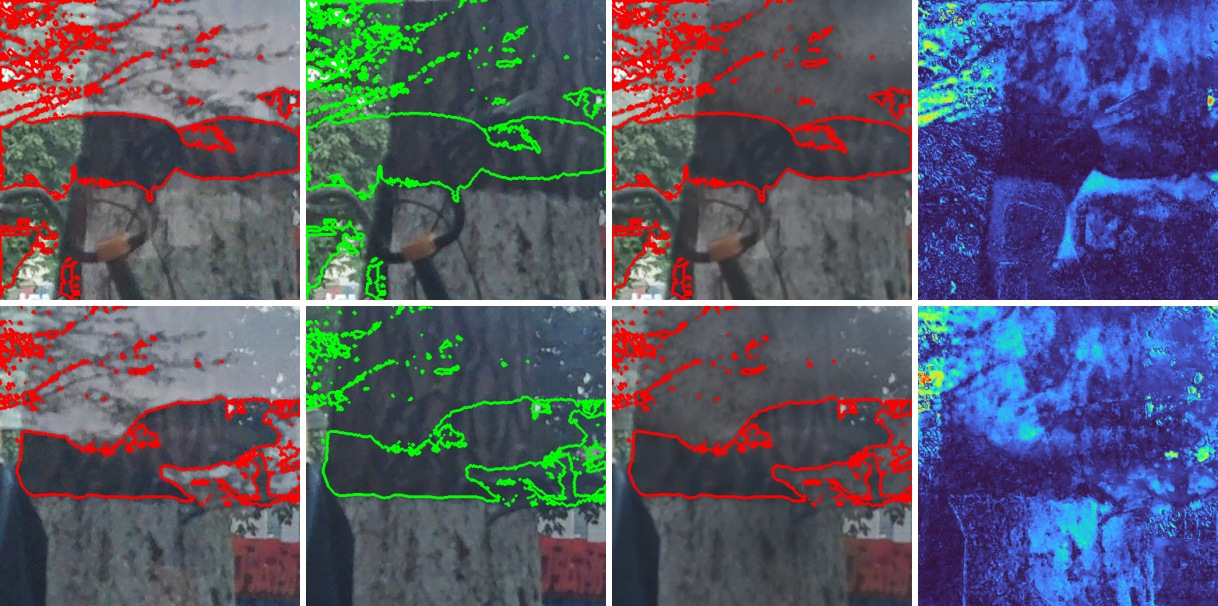
\includegraphics[width=\linewidth]{fig/qual_omega.jpg}
\caption{\textbf{Where the damage happens.} Two scenes (rows). Columns: input $I$; ground
truth $T$; our prediction; absolute error $|\That-T|$ (turbo, per-image normalised).
Red/green contours: the hand-annotated occluder region $\Om$. The error map lights up
\emph{along the occluder} rather than in the reflected content---the signature of a
``remove reflection'' prior applied where there is little reflection to remove.}
\label{fig:qual}
\end{figure}

\subsection{$\Om$ needs almost no change; its \emph{neighbourhood} does}
\label{sec:axis1}

The occluder region $\Om$ is not where the reflection is strongest---it is where it is weakest.
Partitioning each frame into $\Om$, a $15$\,px annulus around it, and the remaining far field gives
three bands that behave completely differently:

\begin{center}
\small
\setlength{\tabcolsep}{3pt}
\begin{tabular}{@{}lccccc@{}}
\toprule
band & area & $\mathbb{E}|I-T|$ & refl./trans. & identity & $+\quiet$ \\
\midrule
$\Om$ itself        & ---    & $\mathbf{10.3}$ & $0.112$ & $24.49$ & $22.26$ ($-2.23$) \\
\textbf{annulus ($15$\,px)} & $44.4\%$ & $\mathbf{44.4}$ & $\mathbf{0.516}$ & $13.76$ & $19.44$ ($\mathbf{+5.68}$) \\
far field           & ---    & $16.8$ & $0.164$ & $19.52$ & $23.53$ ($+4.02$) \\
\bottomrule
\end{tabular}
\end{center}

(PSNR is computed within each band, so bands are not comparable to one another; the informative
quantity is each model against identity \emph{within} a band.)

Three readings. \emph{(a)} The reflection in the annulus is $4.3\times$ stronger than inside $\Om$
and $2.6\times$ stronger than in the far field: the strong reflection does not sit \emph{in} the
occluder region, it sits \emph{next to} it. \emph{(b)} The annulus is not a fringe---it covers
$44\%$ of the frame---and it is where the models' absolute quality is worst ($19.4$--$19.8\dBA$
versus $23.5$ far away). \emph{(c)} Inside $\Om$ every method is worse than doing nothing
($-2.2\dBA$), because almost nothing needs to change there ($10.3$ gray levels) and the model
changes it anyway.

% 中文：这条把"边界为什么显眼"讲清楚——不是 Ω 内坏了，是紧邻的强反射带质量最差，
% 而它贴着 Ω，人眼一对比就看出来了。要修它必须靠长程语义连续（例如左下角的树干下半段）。
The consequence is perceptual rather than numerical: the annulus abuts a region that is already
almost correct, so its residual error is read by the eye as a \emph{boundary}. Fixing it is not a
matter of removing more reflection---the transmitted structure there is buried, and recovering it
requires extrapolating from content elsewhere in the frame along semantic continuations (a tree
trunk continued from its lower part, a railing continued from the left). This is the cloze-like
regime of Sec.~\ref{sec:band}, and it is the one failure mode no method we tested addresses.

\subsection{The damage is structural, and no model beats a blur}
\label{sec:structural}
\label{sec:ceiling}

A photometric explanation would predict that the models merely mis-scale $\Om$. They do
not. Restricting to $\Om$ and allowing a \emph{per-image affine correction} before
scoring, models keep only a fraction of the ground-truth structure:

\begin{center}
\small
\setlength{\tabcolsep}{4pt}
\begin{tabular}{@{}lcccc@{}}
\toprule
 & identity & base & $+\quiet$ & 50:50 \\
\midrule
structure retained (LapVar ratio) & $1.14$ & $0.50$ & $\mathbf{0.65}$ & $0.48$ \\
MAE, per-image affine-corrected & $10.51$ & $12.82$ & $11.70$ & $\mathbf{10.71}$ \\
\bottomrule
\end{tabular}
\end{center}

Two readings. First, the mixed model's affinity-corrected error ($10.71$) is essentially
identity's ($10.51$) while its structure is halved---it ``wins'' the error metric by
flattening $\Om$. Second, we can bound what any content-agnostic method can do: smoothing
the input with a Gaussian is the best a model can achieve if it knows nothing about the
content. On the weakly-reflected $59\%$ of $\Om$ that ceiling is $29.50\dBA$, against
identity's $31.45$ and $\quiet$'s $27.18$; on the strongly-reflected $7\%$ it is
$15.24\dBA$, against $14.46$ (identity) and $13.48$ ($\quiet$). \textbf{No model we
trained beats a plain blur, in either regime.}

\subsection{Reflection and scene share the frequency band}
\label{sec:band}

$34.5\%$ of the reflection's energy lies above a $\sigma{=}8$ low-pass, so it is not a veil
that can be filtered away. We verified the consequence directly: replacing the low
frequencies of a model output with those of the model and the high frequencies with those
of the \emph{input},
$\That' = \mathrm{LP}_\sigma(\That) + \big(I-\mathrm{LP}_\sigma(I)\big)$, inside $\Om$
restores structure fidelity ($1.31\times$ at $\sigma{=}2$) but \emph{lowers} PSNR:

\begin{center}
\small
\setlength{\tabcolsep}{4pt}
\begin{tabular}{@{}lccc@{}}
\toprule
PSNR in $\Om$ & plain & $+\,\sigma{=}2$ & $+\,\sigma{=}4$ \\
\midrule
$+\quiet$ & $22.26$ & $22.04$ & $21.66$ \\
50:50 & $23.73$ & $23.39$ & $22.97$ \\
\bottomrule
\end{tabular}
\end{center}

The band that carries the missing structure also carries the reflection. Separating the
two is not a filtering problem; it requires knowing which structures belong to the scene,
i.e.\ a semantic prior. This is also why a perceptual loss does not help: it is
\emph{mean-seeking}, so under the layer ambiguity of Eq.~\eqref{eq:film} it averages the
plausible completions and produces the conservative ``hedged'' output we observe.

\subsection{What survives fine-tuning is per-image}
\label{sec:photometric}

We measure two photometric oracles: a per-image affine fitted on that image's ground
truth, and a single shared affine fitted on the other $14$ scenes (leave-one-scene-out).
Their gap is the part any cross-scene rule could remove.

\begin{center}
\small
\setlength{\tabcolsep}{4pt}
\begin{tabular}{lcc}
\toprule
 & per-image oracle & shared (LOO) \\
\midrule
identity & $+1.94$ & $+0.50$ \\
RDNet (zero-shot) & $+1.00$ & $+0.59$ \\
ours (fine-tuned) & $+0.15$--$0.26$ & $+0.07$ \\
\bottomrule
\end{tabular}
\end{center}

Fine-tuning consumes the transferable part ($0.59\rightarrow0.07\dBA$) and leaves a
residual that is per-image. Any module estimating a global photometric quantity from a
single frame is therefore bounded by $0.07\dBA$---which is why the $8{\times}8$ adapter and
the input-side rescaling of Sec.~\ref{sec:negative} both failed.

\subsection{The load-bearing term is not about the region}
\label{sec:axis3}

Our loss contains a region-relative error inside $\Om$,
\begin{equation}
\reg=\lambda_{\Om}\,\mathbb{E}_{\Om}\!\left[\,
\frac{|T-\That|}{\mathbb{E}_{\Om}|T-I|}\ \right].
\label{eq:lom}
\end{equation}
Removing it is catastrophic---PSNR falls from $22.49$ to $18.33\dBA$, i.e.\ \emph{below}
identity ($18.44\dBA$)---so by any ablation it is the single most important term of a
nine-term objective. Its power, however, is not the annotation. Replacing the hand mask by
a random disk of equal area (three seeds, separate $82$-pair pool) gives

\begin{center}
\small
\setlength{\tabcolsep}{4pt}
\begin{tabular}{lcc}
\toprule
region used in Eq.~\eqref{eq:lom} & PSNR & seed sd \\
\midrule
none ($\lambda_\Om=0$) & $17.76$ & $0.16$ \\
hand-annotated $\Om$ & $19.41$ & $0.54$ \\
\textbf{random disk} & $\mathbf{19.90}$ & $\mathbf{0.16}$ \\
\bottomrule
\end{tabular}
\end{center}

% 中文：这条说明为什么"紧凑区域 + 高权重"在这里需要而在普通 SIRR 里不需要。
% 注意：这是**由覆盖率统计支撑的推断**，不是在公开数据上训出来的结论，行文里要标明。
\paragraph{Why a compact, high-weight region helps here and not in standard SIRR.}
We do not claim this as a training result on public data; we state it as an inference supported by
coverage statistics. Defining the reflection's spatial \emph{coverage} as the fraction of pixels
whose residual exceeds $15\%$ of its 90th percentile, the median coverage is $83.5\%$ on
SIR$^2$ ($499$ pairs), $70.6\%$ on Real20 ($109$ pairs) and only $52.7\%$ on our filmed panel. When
the reflection covers almost the whole frame, a global $L_1$ already carries a separation signal
everywhere and no extra term is needed. When it covers half the frame, the global loss is dominated
by pixels for which ``do nothing'' is nearly optimal (inside $\Om$, $\mathbb{E}|I-T|=10.3$ gray
levels), and a compact region with a large weight is what puts the gradient back. This is also why
region-weighted losses are routine in \emph{sparse}-degradation restoration---deraining, scratch and
shadow removal---while being essentially absent from the SIRR literature: existing SIRR data is
dense, and there is nothing for them to expose.

A random disk is not only as good, it \emph{stabilises} training. The benefit of
Eq.~\eqref{eq:lom} is the relative normalisation---being accurate in a compact region
despite little change being needed---not region recognition. Sec.~\ref{sec:method} turns
this into a mask-free regularizer.

% ============================================================================
% 中文注释：第 5 节 方法（Method）
% ----------------------------------------------------------------------------
% 这一节只讲两件事：① 保留区域相对误差但去掉"硬掩码"；② 引入 L_quiet。
% 明确不碰架构：底座是强微调的 RDNet（冻结 FocalNet 主干，66M 可训参数，6000 it / bs4）。
% 数学要点：
%   n(x) = 逐像素"本来需要改多少"（训练期用 GT，测试期不需要）
%   w(x) = (1 − n/τ)_+，τ = 0.05
%   L_quiet = λ·E[ w(x)·|T̂(x) − I(x)| ]，λ=1
%   性质：w≡0 时严格退化回基线；不加参数、不加推理成本；只作用在最终输出上。
% 与式 (2) 的关系：两者都是"相对误差 × 需要改动量"；差别是式(2)按区域归一，L_quiet 按像素。
% 诚实点：§6.2 会说明它的收益**不集中在 Ω**，所以不要在这里暗示它能修好遮挡区。
% ============================================================================
\section{Method}
\label{sec:method}

% 中文：底座与配方一句话交代清楚，避免读者以为我们在卖架构。
Our model is a strongly fine-tuned RDNet~\cite{rdnet25} (frozen FocalNet backbone, all other
parameters trainable, $66$M parameters, $6000$ iterations at batch $4$). The contribution of this
paper is not the architecture but \emph{what the loss should ask for}. We describe the two terms
that matter and the one we add.

\subsection{Region-relative error (kept, but no longer masked)}

% 中文：式(2) 是功臣，但 §4.3 证明它的力量来自分母归一，不来自 Ω。所以把硬区域换成逐像素权重。
Eq.~\eqref{eq:lom} is the workhorse. Sec.~\ref{sec:axis3} showed that its power comes from the
normalization by $\mathbb{E}_{\Om}|T-I|$, not from $\Om$. We therefore replace the hard region by a
\emph{smooth per-pixel weight} that plays the same role without any annotation.

% 中文：定义"需要的改动量" n(x)（三通道平均绝对差，只在训练期用 GT 算）。
Define the \emph{needed change}
\begin{equation}
n(x) \;=\; \frac{1}{3}\sum_{c}\big|I_c(x)-T_c(x)\big| \quad (\text{training only}),
\end{equation}
% 中文：改变化感知权重 w(x)：需要改得越少，权重越大。
and the change-aware weight
\begin{equation}
w(x) \;=\; \Big(1-\frac{n(x)}{\tau}\Big)_{+},\qquad \tau=0.05 .
\end{equation}
% 中文：L_quiet 本体——"几乎不需要改的地方，就不要动图像"。
The regularizer is
\begin{equation}
\boxed{\;\quiet=\lambda\,\mathbb{E}\big[\,w(x)\,\big|\That(x)-I(x)\big|\,\big]\;}
\label{eq:quiet}
\end{equation}
% 中文：默认 λ=1；只作用在最终输出上；不加参数、不加推理成本；w≡0 时严格等于基线。
with $\lambda=1$ by default. Intuitively: \emph{where almost nothing needs to change, do not move
the image}. This is exactly what Eq.~\eqref{eq:lom} enforces inside $\Om$, but it is expressed
directly in terms of the supervision signal, so it (a)~needs no mask, (b)~does not assume the
region is compact, and (c)~is well defined on synthetic pairs and on real pairs alike.
$\quiet$ is evaluated on the final output $\That$ only; it adds no parameters and no inference
cost. With $w\equiv0$ the loss reduces exactly to the baseline, so the baseline is a strict special
case.

\subsection{Why this shape}

% 中文：为什么是这个形状——式(5) 是式(2) 的无掩码极限；§4.3 预测逐像素版本应保留收益，§6.2 验证。
Eq.~\eqref{eq:quiet} is the mask-free limit of Eq.~\eqref{eq:lom}: both are ``relative error
weighted by how much change is needed''. The difference is that Eq.~\eqref{eq:lom} measures the
needed change \emph{inside a region} and multiplies the region's contribution by a constant,
whereas Eq.~\eqref{eq:quiet} measures it \emph{per pixel}. The diagnosis of
Sec.~\ref{sec:axis3} predicts that the per-pixel version should retain the benefit, and
Sec.~\ref{sec:exp:quiet} confirms it.

% 中文：反向论证——没有这种信号的模型会退化成"整体压暗"，对应 β≈−0.29 而 α≈1.0。
Conversely, a model that receives no such signal collapses to
``darken everything'', which is what $\beta\approx-0.29$ with $\alpha\approx1.0$ indicates.

\subsection{Full objective}

% 中文：其余 8 项损失保持不动，这样每个对比只隔离一个变量（可复现性）。
The remaining terms (reconstruction consistency $|I-\That-\Rhat|$, a gradient-exclusion term, a
one-sided overshoot hinge, first- and second-order fidelity, DISTS, and a reflection-column term)
are kept unchanged from the baseline for all experiments reported here, so that every comparison
isolates one factor.

% ============================================================================
% 中文注释：第 6 节 实验（Experiments）
% ----------------------------------------------------------------------------
% 五小节：
%   6.1 主表：公开方法 + identity + 我们两臂。注意"我们比最好的公开方法高 +2.0 dB 是靠过平滑
%       换来的"（LapVar 比 0.60）——这一句必须写，否则等于自吹。
%   6.2 L_quiet：三种子 +0.50（CI [+0.34,+0.67]，14/15）；五种子 22.86±0.36；
%       **诚实点**：增益不集中在 Ω（22.30→22.39），所以不主张它修好遮挡区；
%       **不冗余**：去掉区域项只剩 19.53 / 20.26，说明两项互补。
%   6.3 哪一项吃重：区域项 4.16 > 梯度排斥 1.17 > 重建一致 1.12 > hinge 0.37；
%       L_r 原本是死的（分母 bug），按 RDNet 原版复活后单种子 +1.22、三种子 +0.18（噪声内）。
%   6.4 域消融：May 21.79 / Apr 20.72 / Jun(44) 20.57 / Jun(1093) 20.35 / 零样本 20.05。
%       关键解释：1093 对没用是**GT 错位**（88.7% >3px），对齐后 21.43；只筛掉最烂 99 对就 +0.80。
%   6.5 负结果表：两个结构方案是被 41–160 秒的 CPU 探针提前否掉的（省 12 GPU·h）；
%       权重平均 20.78 说明三种子落在不同 basin，种子方差不是噪声。
% 引用注意：所有 PSNR 来自同一冻结评测脚本（读 uint8 PNG），不是训练日志里的浮点值。
% ============================================================================
\section{Experiments}
\label{sec:experiments}

% 中文：统一配方（冻结 FocalNet、6000 it、bs4、30% 真实/40% 在线合成/30% 开源直督），
% 训练池来自 5 月+6 月共 174 对/7 场景；所有数字由同一个评测脚本产出。
\paragraph{Setup.}
Unless stated otherwise all arms use the same recipe: RDNet with a frozen FocalNet backbone,
$6000$ iterations, batch $4$, Adam at $10^{-4}$, random crops $224\!\rightarrow\!256\! \rightarrow\!320$,
$30\%$ real pairs / $40\%$ online-synthesised pairs / $30\%$ public SIRR pairs. Training pools are
built from a $5$-month and a $6$-month capture ($174$ pairs, $7$ scenes). Every number in
Tab.~\ref{tab:main} is produced by the same frozen evaluation script, which reads the stored
uint8 PNG predictions.

\subsection{Main results}

% 中文：两条读法——(a) 所有方法在 Ω 内都是负的，我们只是把伤害从 −3.4 减到 −2.2；
% (b) 我们 +2.0 dB 的领先是靠过平滑换的（LapVar 比 0.60），所以 PSNR 只当一个坐标看。
Tab.~\ref{tab:main}. Two observations.
\emph{(a)} All public methods are more than $3\dBA$ worse than identity inside $\Om$, and the
fine-tuned models reduce that damage to $-2.2\dBA$ without ever becoming safe: the occluder region
remains the region where SIRR hurts, for every method we tested.
\emph{(b)} The aggregate gap between our baseline and the best public method ($+2.0\dBA$) is
obtained at the cost of over-smoothing: the LapVar ratio is $0.60$ for our model (identity $1.0$),
while HF-PSNR and gradient cosine are comparable. We therefore treat PSNR as one coordinate of the
result, not as the result.

\subsection{The change-aware regularizer}
\label{sec:exp:quiet}

% 中文：逐场景 Δ 图——14/15 为正，均值 +0.50，CI [+0.33,+0.67]；唯一为负的场景只有 −0.07（噪声内）。
\begin{figure}[t]
\centering
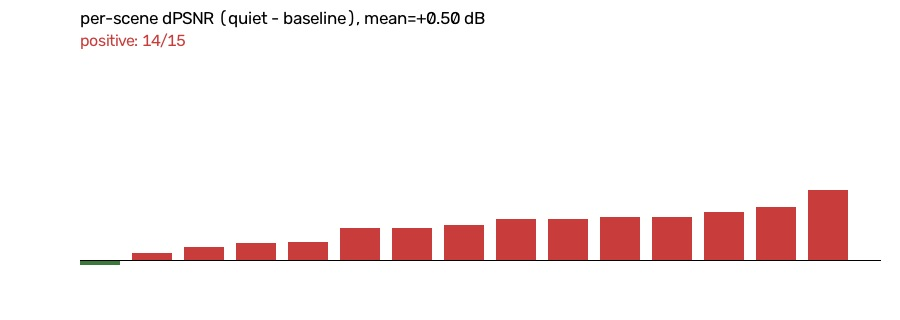
\includegraphics[width=\linewidth]{fig/perscene.jpg}
\caption{\textbf{Per-scene effect of $\quiet$} (mean of three seeds, minus the three-seed
baseline). Bars sorted by gain; $14$ of $15$ scenes improve, mean $+0.50\dBA$, $95\%$ CI
$[+0.33,+0.67]$. The single loss is $-0.07\dBA$, i.e.\ within measurement noise.}
\label{fig:perscene}
\end{figure}

% 中文：三种子 22.99±0.34 vs 基线 22.49±0.44；五种子 22.86±0.36。
% **必须写明种子轴 CI 仍跨 0**——我们只能主张逐场景稳健，不能主张跨种子稳健。
\paragraph{Seeds.} $\quiet$ ($\lambda=1$, $\tau=0.05$) gives $22.99\pm0.34$ over three seeds
($22.71/23.38/22.88$) versus $22.49\pm0.44$ for the baseline ($21.99/22.84/22.62$). The paired
per-scene improvement is $+0.50\dBA$ with a $95\%$ CI of $[+0.34,+0.67]$ and is positive on
$14/15$ scenes; a five-seed run gives $22.86\pm0.36$. The \emph{seed-level} interval, however, still
contains zero ($[-0.07,+1.08]$): with three seeds we can claim per-scene robustness but not
seed-level robustness, and we report it as such.

% 中文：λ=5 反而略低（+0.44）但 15/15 全正、种子方差最小 ⇒ 它更像"约束"而非"新目标"。
\paragraph{Strength.} $\lambda=5$ gives $+0.44\dBA$ with $15/15$ scenes positive and the smallest
seed spread ($22.92\pm0.16$). Increasing $\lambda$ does not give more, which is consistent with the
regularizer acting as a \emph{constraint} rather than as an additional objective.

% 中文：诚实点——收益**不**集中在 Ω（22.30→22.39，仅 +0.09），所以不主张它解决遮挡区问题；
% 它阻止的是"在不该动的地方动"，效果摊在全图上。
\paragraph{It is not a region fix.} The gain is \emph{not} concentrated inside $\Om$
($22.30\rightarrow22.39\dBA$, i.e.\ $+0.09$), so we explicitly do not claim that $\quiet$ solves
the occluder problem of Sec.~\ref{sec:axis1}. What it does is prevent the model from moving pixels
that need no change; the benefit is spread over the whole frame, and the fourteen scenes that gain
do so on non-$\Om$ content.

% 中文：但也不冗余——把区域项关掉只留 L_quiet，只有 19.53（连 hinge 也关掉是 20.26），
% 远低于两者同时用的 22.99。⇒ 区域项供大头，L_quiet 追加增量。
\paragraph{It is not redundant with the masked term.} Removing the annotation entirely and keeping
only $\quiet$ is much worse than keeping both: with $\lambda_\Om=0$ and $\quiet$ active the panel
score is $19.53\dBA$ (and $20.26\dBA$ if the hinge term is also disabled), against $18.33\dBA$ for
$\lambda_\Om=0$ alone and $22.99\dBA$ for the full model. The two terms are therefore
\emph{complementary}: Eq.~\eqref{eq:lom} supplies the bulk, $\quiet$ adds the rest.

\subsection{Which loss terms are load-bearing}

% 中文：留一法（单种子、同池）。区域项 4.16 最大；梯度排斥 1.17；重建一致 1.12；hinge 0.37；
% L_r 原本数值上是死的（分母多乘 hw），按 RDNet 原版复活后单种子 +1.22 但三种子只有 +0.18（噪声内）。
We remove one term at a time from the nine-term objective (single seed, same pool). Removing the
reconstruction consistency $|I-\That-\Rhat|$ costs $1.12\dBA$; removing the gradient-exclusion term
costs $1.17\dBA$; removing the overshoot hinge costs $0.37\dBA$; the region term costs
$4.16\dBA$ (Sec.~\ref{sec:axis3}). The reflection-column term contributes $+0.02\dBA$---we later
found it had been numerically dead (a normalisation bug) and that reviving it in RDNet's original
squared form yields $+1.22\dBA$ on one seed but only $+0.18\dBA$ over three ($23.21/22.51/22.27$),
i.e.\ inside the seed spread. DISTS and the Laplacian fidelity term contribute $+0.08$ and
$+0.07\dBA$. This ordering is stable across pools.

\subsection{Domain ablation: what makes a real pair useful?}

% 中文：同配方换域：May 21.79 / Apr 20.72 / Jun(2 场景,44 对) 20.57 / Jun(13 场景,1093 对) 20.35，
% 零样本 20.05 ⇒ **1093 对等于白给**，与样本量直觉相反。
\paragraph{Domain ablation.}
Training the same recipe on different capture months, one domain at a time, gives
$21.79$ (May), $20.72$ (April), $20.57$ (June, $2$ scenes) and $20.35$ (June, $1093$ pairs,
$13$ scenes) against $20.05$ for the zero-shot model. A $1093$-pair pool is thus worth
\emph{nothing}, which is the opposite of what its size suggests.

% 中文：原因不是域漂移，是**几何错位**：88.7% 的对位移 >3px（中位 8.2px），因为 T 是手持片段最后一帧。
% 对齐后 21.43；只丢掉最烂的 99 对就已从 20.35 升到 21.15。⇒ GT 对齐是 SIRR 训练数据的一阶属性。
The cause is not domain shift:
phase correlation shows that $88.7\%$ of those pairs have $T$ misaligned with $I$ by more than
$3$\,px (median $8.2$\,px), because $T$ is the last frame of a handheld clip. After per-pair
translation alignment the same pool reaches $21.43\dBA$ (single seed), and merely \emph{discarding
the worst $99$ pairs} already improves the unaligned pool from $20.35$ to $21.15\dBA$. Ground-truth
alignment is therefore a first-order property of SIRR training data, and we recommend reporting the
alignment distribution alongside the pair count.

% 中文：混训的结果——Ω 抬上去了，但 β 掉下来，说明是"少动"不是"学会补图"。
\paragraph{Mixing occluder-rich data improves $\Om$ but not the task.}
Since the occluder region is where models fail, one may try to fix it with data. Mixing
our $11$-month indoor capture into the $5{+}6$-month pool raises $\mathrm{PSNR}_\Om$ from
$20.91$ to $23.76\dBA$ at a $50{:}50$ ratio, and the gain is broad---positive on
$15/15$ scenes, mean $+2.84\dBA$. It is also misleading: the same arm moves from $\beta=-0.34$
to $-0.47$ and its action ratio (mean $|\That-I|$ over mean $|I-T|$) drops from $0.79$ to
$0.60$, i.e.\ it wins $\Om$ by \emph{doing less}. At $75\%$ the pool reaches
$\mathrm{PSNR}_\Om=23.78$ with $\beta=-0.63$ and an action ratio of $0.43$. No mixture
beats the best single-domain model on the full metric ($22.38$ vs.\ $22.71$), so we read
this as further evidence that $\mathrm{PSNR}_\Om$ alone does not identify progress.

\subsection{Negative results}
\label{sec:negative}

% ============================================================================
% 中文注释：表 2 负结果（单栏）
% ----------------------------------------------------------------------------
% 三组，用横线隔开：
%   ① 针对 Ω 内容恢复的尝试（全部失败，且**都能从 §4.3 的"同频段"解释**）
%       感知损失（LPIPS/GAN 式）—— 对冲求稳：mean-seeking，多解时取平均
%       把输入高频拼回 Ω —— 结构回到 1.31×，但 PSNR 掉 0.22–0.31 dB（把反射也搬回来了）
%       加遮挡区数据混训 —— Ω 抬 +2.84 dB（15/15），但 β 从 −0.34 退化到 −0.47、
%                              动作比 0.79→0.60：是"少动"不是"学会补图"
%   ② 真的训练过的其它臂
%   ③ 被 CPU 探针提前否掉的（省 GPU 时）
% 注意：这张表不是"实验失败记录"，而是"哪条路已被证否"的证据；不要因为都是负的而删。
% ============================================================================
\begin{table}[t]
\centering
\caption{Negative results. ``Probe'' rows were rejected by a CPU-only learnability probe
before any training run. The first block are attempts to \emph{recover the content of
$\Om$}; all fail, and Sec.~\ref{sec:band} explains why.}
\label{tab:negative}
\footnotesize
\setlength{\tabcolsep}{3pt}
\begin{tabular}{@{}p{0.48\linewidth}p{0.46\linewidth}@{}}
\toprule
Proposal & Result / verdict \\
\midrule
perceptual loss inside $\Om$ & hedged / averaged, no gain \\
splice input $\mathrm{HF}$ into $\Om$ & $-$0.22 (struct.\ $1.31\times$) \\
mix $25$--$50\%$ occluder data & $\Om$ $+2.84$ but $\beta$ $-0.34\!\to\!-0.47$ \\
extra synthetic pairs & $22.34$ vs $22.38$, null \\
\midrule
$8{\times}8$ photometric adapter ($+18$k) & $-0.06$, fail (3 seeds) \\
input-side rescaling to match $g$ & $+0.19$, null (1 seed) \\
reweight gradient fidelity & $-0.18$, \emph{worse} \\
region-agnostic loss shift & $-0.34$, useful (kept) \\
deeper $L_1$ on reflection column & $+0.34$, below gate \\
final iterations with MSE & $+0.28$, below gate \\
\midrule
dual-dict.\ proximal separation & probe $-0.08$..$-0.26$, rejected \\
residual-magnitude gate ($1025$ par.) & probe $-0.29$, rejected \\
weight averaging of 3 seeds & $20.78$, fails (basins) \\
\bottomrule
\end{tabular}
\end{table}


% 中文：两点——① 三个结构方案都是被 41–160 秒的 CPU 探针提前否掉的（各省 6 GPU·h），
% 在效应量只有 ~0.3 dB、种子方差 0.44 的情况下，这种探针应当成为强制流程；
% ② 三种子权重平均 20.78 < 任一成员，说明种子落在不同 basin，观测到的方差不是"同一解附近的噪声"。
Tab.~\ref{tab:negative} lists proposals that did not work. Two comments. First, the
\emph{structural} proposals (a photometric adapter of $18$k parameters, a residual-magnitude gate
of $1025$ parameters, a dual-dictionary proximal layer separation) were all falsified by a
\emph{CPU-only probe}: fit the candidate's last layer on training scenes and evaluate on held-out
scenes. The probes take $41$--$160$ seconds and each saved a $6$ GPU-hour training run. Given that
the effect sizes we can resolve are $O(0.3\dBA)$ and the seed spread is $0.44\dBA$, we consider such
probes mandatory rather than optional. Second, weight averaging of three seeds fails catastrophically
($20.78\dBA$, i.e.\ below any of its constituents): the seeds sit in different basins, so the
per-scene variance we observe is \emph{not} noise around a common solution.

% ============================================================================
% 中文注释：第 7 节 讨论与局限（Discussion and Limitations）
% ----------------------------------------------------------------------------
% 这一节的作用是"主动交代短板"，比被审稿人问出来好：
%   ① 面板只有 15 场景、单一地点，而且**开发过程中用过** ⇒ 是开发集，不是确认集。
%   ② 统计功效：15 场景、种子 sd 0.44 ⇒ 场景轴 MDE≈0.26 dB，种子轴≈1 dB；
%      所以 +0.50 只能算"场景层面证据"。
%   ③ 余量在哪：光度已被吃干（0.07）、区域项改进不了（换掩码无效）、L_quiet 只 +0.50；
%      剩下的全是数据问题（对齐 + 锁曝光 + Ω 标注 + 场景数）。
%   ④ 六条采集 checklist（这是本文对社区最实用的产出之一）。
%   ⑤ 诚实声明：不主张 PSNR 胜出；Ω 内的差距可能本质上不可解（拍摄者就是遮挡者）。
% ============================================================================
\section{Discussion and Limitations}
\label{sec:conclusion}

% 中文：面板小、单地点、开发期用过 ⇒ 只能当开发集。给出两条 MDE，说明我们为什么只主张场景层面。
\paragraph{What the community should measure.}
Our panel is small ($15$ scenes) and single-site, and it was used during the development of the
regularizer, so it is a development set, not a confirmatory one. With $15$ scenes and a seed spread
of $0.44\dBA$, the minimum detectable effect at $95\%$ confidence is about $0.26\dBA$ \emph{per
scene} but roughly $1\dBA$ at the seed level: any claim below that is a claim about one seed. We
therefore report the seed interval everywhere and treat our own $+0.50\dBA$ as scene-level evidence.

% 中文：余量盘点——光度 0.07 已饱和、区域项换掩码无效、L_quiet 只 +0.50；
% 所以"更大的网络/新注意力/新门控"大概率不动这个面板，瓶颈是数据。
\paragraph{Where the headroom is --- and is not.}
Photometric headroom is exhausted ($\Delta_{\mathrm{aff}}=0.15$--$0.26$, shared
$0.07\dBA$), the region term cannot be improved by a better mask, and the change-aware term
adds $0.50\dBA$. The obvious next lever, data, does not work either: mixing occluder-rich
frames raises $\mathrm{PSNR}_\Om$ by $+2.84\dBA$ on every scene while $\beta$ degrades from
$-0.34$ to $-0.47$, because the model simply moves less. What is left is the layer
ambiguity of Eq.~\eqref{eq:film}: inside $\Om$ the reflection and the scene occupy the same
frequency band, so restoring the input's high frequencies lowers PSNR and a perceptual
loss hedges. We see no evidence that a larger network, a new attention block or a new gate
would move this panel. Faithful recovery of $\Om$ looks like a conditional-completion
problem and will need semantic priors that are \emph{long-range}, not local or
statistical---the kind a human uses when reading the continuation of a wall or a railing
behind an occluder. We state this as an open problem, not as a result.

% 中文：六条采集 checklist——这是本文最可直接复用的产出（锁曝光、相机别动、报对齐分布、
% 报场景数与 GT 数、标 Ω、说明反射源是"被移走"还是"被遮挡"）。
\paragraph{A checklist derived from the failures.}
From the failure modes in Sec.~\ref{sec:benchmark} and Sec.~\ref{sec:negative} we distill a short
checklist for SIRR data collection: (1)~lock exposure and white balance; (2)~do not move the
camera between $I$ and $T$---if you must, record a reference frame and align; (3)~report the
alignment distribution, not only the pair count; (4)~report one ground truth per scene and say how
many independent scenes the pool has; (5)~annotate the occluder region once per scene and report
metrics inside it; (6)~state whether the reflection source was physically removed, because that
changes the illumination of the transmitted layer.

% 中文：诚实声明——本文不主张 PSNR 胜出；Ω 内与 identity 的差距可能本质上不可解
% （采集者本人就是遮挡者，单帧未必含足够信息把"这块暗是拍摄者"和"这块暗是场景"分开）。
\paragraph{Honest statement.}
This paper does not propose a method that wins on average PSNR. It reports that the standard
protocol hides a systematic failure, supplies a measurement of that failure, and derives a small
fix which is statistically supported at the scene level and negligible in cost. The remaining
discrepancy between our models and identity \emph{inside} the occluder region is unexplained and
may be irreducible: the collector of the data is the occluder, and a single frame arguably does not
contain the information needed to tell ``this dark patch is the photographer'' from ``this dark
patch is the scene''.


{
    \small
    \bibliographystyle{ieeenat_fullname}
    \bibliography{refs}
}

\end{document}
